%% Auto-generated by fig_qualitative.py -- do not edit by hand.
\documentclass[border=0pt]{standalone}
\usepackage{iftex}
\ifPDFTeX
  \usepackage[T1]{fontenc}\usepackage{times}
\else
  \usepackage{fontspec}\setmainfont{texgyretermes}[Extension=.otf,UprightFont=*-regular,BoldFont=*-bold,ItalicFont=*-italic,BoldItalicFont=*-bolditalic]
\fi
\usepackage{graphicx}
\usepackage{tikz}
% Shared method colors for all figures/diagrams (same hexes as figures/src/figstyle.py).
% Validated colorblind-safe on white (all-pairs CVD dE >= 9.4, contrast >= 3.4:1); always pair with a
% second cue (marker shape, label) so identity never relies on hue alone.
\definecolor{cOurs}{HTML}{256ABF}      % KalSea (gate + Kalman forecaster + predictor-corrector gap smoothing)
\definecolor{cKalSea}{HTML}{199E70}    % KalSea (Kalman forecasting, no smoothing)
\definecolor{cSeaCache}{HTML}{D95926}  % SeaCache (SEA gate + residual reuse)
\definecolor{cReference}{HTML}{0B0B0B} % 50-step reference
\definecolor{cInk}{HTML}{0B0B0B}
\definecolor{cInkTwo}{HTML}{52514E}
\definecolor{cMuted}{HTML}{898781}
\definecolor{cGrid}{HTML}{E1E0D9}

\newcommand{\hdr}{\fontsize{7.5}{8.5}\selectfont}
\newcommand{\sub}{\fontsize{7}{8}\selectfont\color{cInkTwo}}
\newcommand{\prm}{\fontsize{7}{8.1}\selectfont\itshape\color{cInk}}
\newcommand{\num}{\fontsize{7}{8}\selectfont\color{cInk}}
\begin{document}
\begin{tikzpicture}[x=1bp,y=1bp,line join=round]
\path[use as bounding box] (0,0) rectangle (495.00,-169.75);
\node[anchor=south,inner sep=0] at (49.08,-21.80) {\hdr Reference};
\node[anchor=south,inner sep=0] at (49.08,-11.40) {\sub 50 NFE};
\draw[cMuted,line width=0.4bp] (11.00,-12.40) -- (87.17,-12.40);
\node[anchor=south,inner sep=0] at (168.58,-11.40) {\sub 13 NFE, identical computed steps};
\draw[cMuted,line width=0.4bp] (90.67,-12.40) -- (246.50,-12.40);
\node[anchor=south,inner sep=0] (h01) at (131.75,-21.80) {\hdr SeaCache};
\path (h01.west) ++(-4.0,1.9) coordinate (mk);
\begin{scope}[shift={(mk)}]\fill[cSeaCache] (-2.10,-2.10) rectangle (2.10,2.10);\end{scope}
\node[anchor=south,inner sep=0] (h02) at (211.42,-21.80) {\hdr KalSea};
\path (h02.west) ++(-4.0,1.9) coordinate (mk);
\begin{scope}[shift={(mk)}]\fill[cOurs] (0.00,-0.25) circle (2.21);\end{scope}
\node[anchor=south,inner sep=0] at (296.58,-21.80) {\hdr Reference};
\node[anchor=south,inner sep=0] at (296.58,-11.40) {\sub 50 NFE};
\draw[cMuted,line width=0.4bp] (258.50,-12.40) -- (334.67,-12.40);
\node[anchor=south,inner sep=0] at (416.08,-11.40) {\sub 13 NFE, identical computed steps};
\draw[cMuted,line width=0.4bp] (338.17,-12.40) -- (494.00,-12.40);
\node[anchor=south,inner sep=0] (h11) at (379.25,-21.80) {\hdr SeaCache};
\path (h11.west) ++(-4.0,1.9) coordinate (mk);
\begin{scope}[shift={(mk)}]\fill[cSeaCache] (-2.10,-2.10) rectangle (2.10,2.10);\end{scope}
\node[anchor=south,inner sep=0] (h12) at (458.92,-21.80) {\hdr KalSea};
\path (h12.west) ++(-4.0,1.9) coordinate (mk);
\begin{scope}[shift={(mk)}]\fill[cOurs] (0.00,-0.25) circle (2.21);\end{scope}
\node[anchor=south west,inner sep=0,text width=237.50bp,align=flush left,font=\prm] at (10.00,-40.50) {``A couch on the left of a chair.''};
\node[anchor=north west,inner sep=0] at (10.00,-42.50) {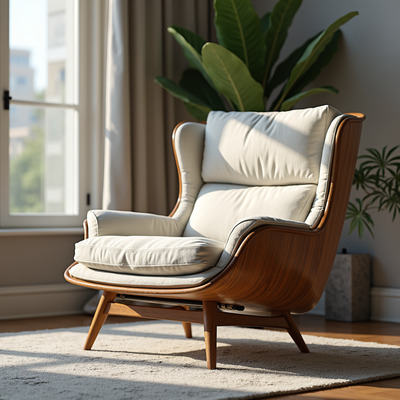
\includegraphics[width=78.167bp,height=78.167bp]{qual_tiles/nfe13_teaser/125_reference_full.jpg}};
\draw[black,line width=1.3bp] (28.32,-94.41) rectangle (47.86,-104.18);
\draw[white,line width=0.6bp] (28.32,-94.41) rectangle (47.86,-104.18);
\node[anchor=north west,inner sep=0] at (10.00,-122.17) {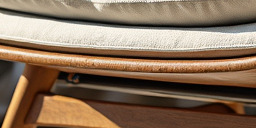
\includegraphics[width=78.167bp,height=39.083bp]{qual_tiles/nfe13_teaser/125_reference_crop.jpg}};
\node[anchor=north,inner sep=0] at (49.08,-163.05) {\num\color{cInkTwo}PSNR (dB)};
\node[anchor=north west,inner sep=0] at (89.67,-42.50) {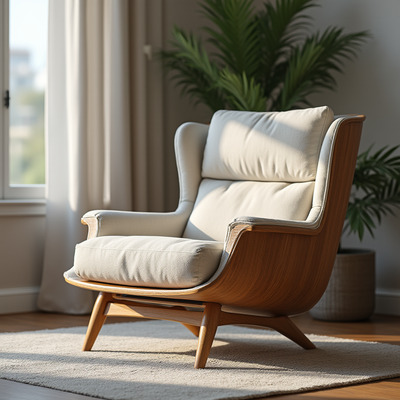
\includegraphics[width=78.167bp,height=78.167bp]{qual_tiles/nfe13_teaser/125_seacache_full.jpg}};
\draw[black,line width=1.3bp] (107.99,-94.41) rectangle (127.53,-104.18);
\draw[white,line width=0.6bp] (107.99,-94.41) rectangle (127.53,-104.18);
\node[anchor=north west,inner sep=0] at (89.67,-122.17) {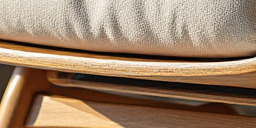
\includegraphics[width=78.167bp,height=39.083bp]{qual_tiles/nfe13_teaser/125_seacache_crop.jpg}};
\node[anchor=north,inner sep=0] at (128.75,-163.05) {\num 19.09};
\node[anchor=north west,inner sep=0] at (169.33,-42.50) {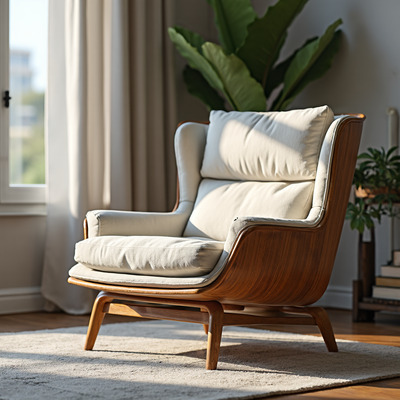
\includegraphics[width=78.167bp,height=78.167bp]{qual_tiles/nfe13_teaser/125_ours_full.jpg}};
\draw[black,line width=1.3bp] (187.65,-94.41) rectangle (207.20,-104.18);
\draw[white,line width=0.6bp] (187.65,-94.41) rectangle (207.20,-104.18);
\node[anchor=north west,inner sep=0] at (169.33,-122.17) {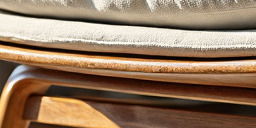
\includegraphics[width=78.167bp,height=39.083bp]{qual_tiles/nfe13_teaser/125_ours_crop.jpg}};
\node[anchor=north,inner sep=0] at (208.42,-163.05) {\num \textbf{20.27}};
\node[rotate=90,anchor=south,inner sep=0] at (6.80,-101.88) {\sub Median gain};
\node[anchor=south west,inner sep=0,text width=237.50bp,align=flush left,font=\prm] at (257.50,-40.50) {``Four cars on the street.''};
\node[anchor=north west,inner sep=0] at (257.50,-42.50) {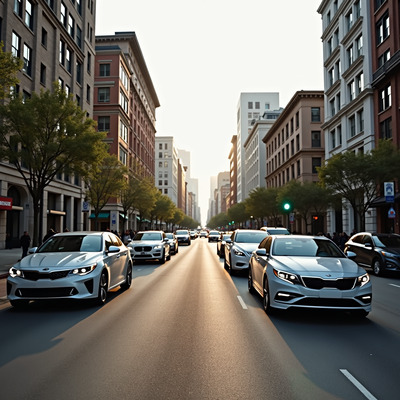
\includegraphics[width=78.167bp,height=78.167bp]{qual_tiles/nfe13_teaser/038_reference_full.jpg}};
\draw[black,line width=1.3bp] (314.90,-52.88) rectangle (334.45,-62.65);
\draw[white,line width=0.6bp] (314.90,-52.88) rectangle (334.45,-62.65);
\node[anchor=north west,inner sep=0] at (257.50,-122.17) {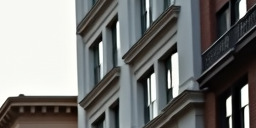
\includegraphics[width=78.167bp,height=39.083bp]{qual_tiles/nfe13_teaser/038_reference_crop.jpg}};
\node[anchor=north,inner sep=0] at (296.58,-163.05) {\num\color{cInkTwo}PSNR (dB)};
\node[anchor=north west,inner sep=0] at (337.17,-42.50) {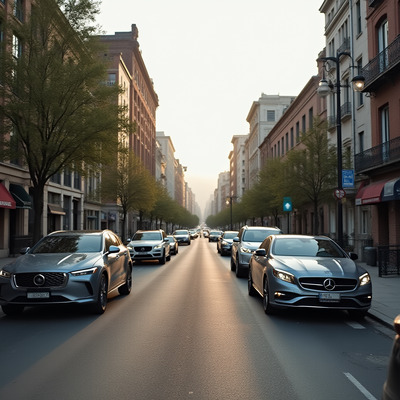
\includegraphics[width=78.167bp,height=78.167bp]{qual_tiles/nfe13_teaser/038_seacache_full.jpg}};
\draw[black,line width=1.3bp] (394.57,-52.88) rectangle (414.11,-62.65);
\draw[white,line width=0.6bp] (394.57,-52.88) rectangle (414.11,-62.65);
\node[anchor=north west,inner sep=0] at (337.17,-122.17) {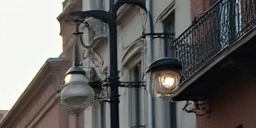
\includegraphics[width=78.167bp,height=39.083bp]{qual_tiles/nfe13_teaser/038_seacache_crop.jpg}};
\node[anchor=north,inner sep=0] at (376.25,-163.05) {\num 16.77};
\node[anchor=north west,inner sep=0] at (416.83,-42.50) {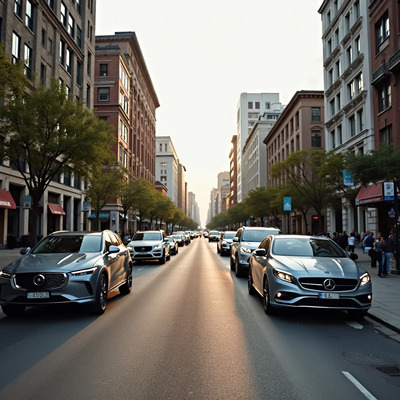
\includegraphics[width=78.167bp,height=78.167bp]{qual_tiles/nfe13_teaser/038_ours_full.jpg}};
\draw[black,line width=1.3bp] (474.24,-52.88) rectangle (493.78,-62.65);
\draw[white,line width=0.6bp] (474.24,-52.88) rectangle (493.78,-62.65);
\node[anchor=north west,inner sep=0] at (416.83,-122.17) {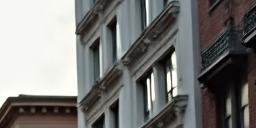
\includegraphics[width=78.167bp,height=39.083bp]{qual_tiles/nfe13_teaser/038_ours_crop.jpg}};
\node[anchor=north,inner sep=0] at (455.92,-163.05) {\num \textbf{19.16}};
\node[rotate=90,anchor=south,inner sep=0] at (254.30,-101.88) {\sub Upper-quartile gain};
\end{tikzpicture}
\end{document}
